\section{Niet-topologische functies}
\label{sec:niet_topologische_functies}
De niet-topologische functies binnen GeoSPARQL zijn beperkter in hoeveelheid, ten opzichte van de topologische functies. In plaats van het onderscheiden van vormen zorgen deze functies voor het uitvoeren van berekeningen. Dit kan bijvoorbeeld het opzoeken van de kortste afstand tussen twee vormen zijn of het samenvoegen van twee vormen om vervolgens een topologische functie erop los te laten. Aan deze functies wordt iets minder aandacht besteed dan aan de topologische functies, omdat deze duidelijk minder gebruikt zullen worden. Toch is er een implementatie gemaakt voor de ``union'' en ``intersection'' functies. De ``union'' functie zal twee vormen samenvoegen tot één nieuwe vorm. De ``intersection'' functie zal dan weer kijken naar het deel dat twee vormen gemeenschappelijk hebben en dit teruggeven. 

Voor het maken van deze implementaties is opnieuw gebruik gemaakt van Turf en dankzij de implementatie van sparqlee, die excellent gebruik maakt van het \textit{divide-and-conquer} (= verdeel en heers) programmeer principe, is deze implementatie op bijna identiek dezelfde manier als de topologische functies mogelijk.

\subsection{Beperkingen}
Aangezien gebruik gemaakt wordt van Turf, moet de manier van Turf gevolgd worden. Hierbij is het enkel mogelijk om de unie of intersectie te berekenen van polygonen. GeoSPARQL beschrijft echter dat deze functies beiden een geometrisch object terug moeten geven die alle punten representeert van het resultaat van deze functies. Dit impliceert dat het ook mogelijk moet zijn om deze functies toe te passen op punten en lijnen. Dit zou zelfs mogelijk moeten zijn voor de combinatie van punten, lijnen en polygonen.

\begin{figure}
    \centering
    \begin{subfigure}[t]{0.5\linewidth}
        \centering
        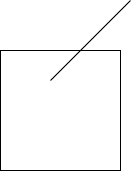
\includegraphics[width=0.3\linewidth]{images/union_example1.png}
        \caption{Voor union.}
        \label{fig:union_example1}
    \end{subfigure}%
    ~ 
    \begin{subfigure}[t]{0.5\linewidth}
        \centering
        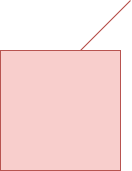
\includegraphics[width=0.3\linewidth]{images/union_example2.png}
        \caption{Resultaat union.}
        \label{fig:union_example2}
    \end{subfigure}
    \caption{Problematiek union.}
\end{figure}

Dit laatste is echter niet mogelijk met de huidige implementatie waar gebruik gemaakt wordt van ``Point'', ``MultiPoint'', ``LineString'', ``MultiLineString'', ``Polygon'' en ``MultiPolygon''. In \figureref{fig:union_example1} is een voorbeeld te zien van twee vormen waarvan de unie (= de vorm die alle punten van beide figuren samen bevat) genomen wordt. In \figureref{fig:union_example2} wordt aangetoond dat het resultaat van de unie van een ``LineString'' en een ``Polygon'' niet te representeren valt in één van de zes eerder genoemde vormen. Hiervoor zou gewerkt moeten worden met een soort ``GeometryCollection''.